\documentclass[10pt]{article}
\usepackage[dvipdfmx]{graphicx}
\usepackage{titlesec}
\usepackage{scrextend}
\usepackage{enumitem}
\usepackage{geometry}
\geometry{margin=1in}
\usepackage[style=authoryear]{biblatex}
\usepackage[dvipdfmx]{hyperref}
\nocite{*}

\hypersetup{
  colorlinks=true,
  linkcolor=black,
  citecolor=black,
  urlcolor=black,
}

\urlstyle{same}
\titleformat{\section}{\Large\sffamily\bfseries}{}{0em}{}[\titlerule]

\begin{document}
\setcounter{secnumdepth}{0}
\setlength{\parindent}{0pt}
\setlength{\baselineskip}{12pt}
\pagestyle{empty}

\begin{minipage}[h]{11cm}
  {\huge\sf\textbf{Ryubu Hosoki}\par}
  \vspace{2mm}
  {\large\sf\textbf{Ph.D. student}\par}
  \vspace{2mm}
  \begin{minipage}[t]{6cm}
    \begin{description}[align=left,leftmargin=1.5cm,style=multiline]
      \setlength{\itemsep}{0pt}
      \item [Phone] +81 90 6462 7532
      \item [Email] hosoki.r.aa@m.titech.ac.jp
    \end{description}
  \end{minipage}
  \begin{minipage}[t]{5cm}
    \begin{description}[align=left,leftmargin=1.8cm,style=multiline]
      \setlength{\itemsep}{0pt}
      \item [Github] \href{https://github.com/Ryb7532}{@Ryb7532}
      \item [Address] Tokyo, Japan
      % \item [Twitter] \href{https://twitter.com/ryubu_hosoki}{@ryubu\_hosoki}
    \end{description}
  \end{minipage}
  \begin{description}[align=left,leftmargin=2cm,style=multiline]
    \setlength{\itemsep}{0pt}
    \item [Research Interests] Distributed Deep Learning, Model Parallelism, Pipeline Parallelism, Tensor Parallelism, 3D Parallelism, Auto-partitioning of DNN Model
  \end{description}
\end{minipage}
\begin{minipage}[h]{5.5cm}
  \raggedleft
  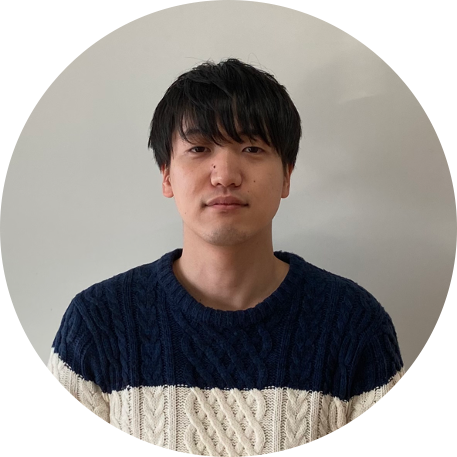
\includegraphics[width=4cm]{./images/icon.png}
\end{minipage}


\section{Education}
\begin{description}[align=left,leftmargin=3.5cm,style=multiline]
  \item[2023.4 -] {\bf Ph.D. Mathematical and Computing Science, Tokyo Institute of Technology, Tokyo, Japan.}
  \item[2021.4 - 2023.3] {\bf Master of Science, Tokyo Institute of Technology, Tokyo, Japan.}\\ GPA: 3.43/4.50
  \item[2017.4 - 2021.3] {\bf Bachelor of Science, Tokyo Institute of Technology, Tokyo, Japan.}\\ GPA: 2.88/4.50
\end{description}


\section{Employment History}
\begin{description}[align=left,leftmargin=3.5cm,style=multiline]
  \item[2023.06 - 2023.08] The French Alternative Energies and Atomic Energy Commission (CEA), Saclay, Research Internship.
  \item[2023.04 -] Tokyo Institute of Technology, Global Scientific Information and Computing Center, Research Assistant.
  \item[2023.04 -] Institute of Physical and Chemical Research (RIKEN), Kobe, Junior Research Associate (declined).
  \item[2021.07 - 2023.03] National Institute of Advanced Industrial Science and Technology (AIST), Tokyo, Research Assistant.
\end{description}


\section{Scholarships}
\begin{description}[align=left,leftmargin=2.5cm,style=multiline]
  \item[2023.04 -] Cross the border! Tokyo Tech Pioneering Doctoral Research Project, Covering living expenses.
  \item[2023.04 -] Tokyo Tech Tsubame Scholarship for Doctoral Students, Covering living expenses (declined).
\end{description}


\section{Teaching}
\begin{description}[align=left,leftmargin=1.2cm,style=multiline]
  \item[2023] Computer Systems, Tokyo Institute of Technology, Math. and Comp. Science, TA.
\end{description}


\section{Publications}
\subsection{Conference Proceedings}
\begin{description}[align=left,leftmargin=0.5cm,style=multiline]
  \item[1.] 
  {\bf Ryubu Hosoki}, Toshio Endo, Takahiro Hirofuchi, Tsutmu Ikegami. "AshPipe: Asynchronous Hybrid Pipeline Parallel for DNN Training." Proceedings of the International Conference on High Performance Computing in Asia-Pacific Region (HPC Asia 2024), pp.117-126, Nagoya, January 2024. {\small DOI: \href{https://dl.acm.org/doi/10.1145/3635035.3635045}{10.1145/3635035.3635045}}
\end{description}

\subsection{Domestic Workshop (Unrefereed)}
\begin{description}[align=left,leftmargin=0.5cm,style=multiline]
  \item[1.] IPSJ SIG Technical Report, 2021-HPC-180, No.9, online, July 2021. (First author)
  \item[2.] IPSJ SIG Technical Report, 2022-HPC-185, No.16, Shimonoseki, July 2022. (First author)
\end{description}


\section{Skills}
\begin{description}[align=left,leftmargin=2.5cm,style=multiline]
  \setlength{\itemsep}{0pt}
  \item [Languages] Japanese (native), English (intermediate)
  \item [Coding] \LaTeX, C/C++, Python, Scala, Ruby, Linux
\end{description}
\end{document}